\pdfminorversion=6 % this is needed to be able to include pdf 1.6. 
                    % For some reasons some old HPSG proceedings have pdf 1.6
\documentclass[11pt,a4paper,fleqn]{article}
\usepackage{times}
\thispagestyle{empty}



\usepackage[T1]{fontenc}   % Silbentrennung

\usepackage[utf8x]{inputenc}
                                                                                                                             
\hyphenation{Acad-e-my}

\usepackage[bookmarks=true,bookmarksopen=true,%
breaklinks=true,%
draft=false,plainpages=false,hyperfootnotes=false,%
pdfauthor={Stefan Müller (Editor)},%
pdftitle={Proceedings of the 10th International Conference on Head-Driven Phrase Structure Grammar},%
pdfkeywords={HPSG}%,
pdftex=true%
%ps2pdf=true  %ohne diesen Treiber geht der Zeilenumbruch in URLs
]{hyperref}% for pdf files
\hypersetup{colorlinks=false, pdfborder={0 0 0}}

\usepackage{pdfpages}
\pdfinclusioncopyfonts=1

\usepackage{orcidlink}

\newcommand\formatauthor[2]{\begin{tabular}[t]{@{}c@{}}
  {\LARGE#1\strut}\\
  {\small#2\strut}\\
  \rule{\dimexpr0.5\linewidth-1em}{0pt}
  \end{tabular}\xhfill\ignorespaces}
\newcommand\xhfill{\hspace{1em plus 1fill}}

\begin{document}

\begin{center}
{\Large
                {\bfseries Proceedings of the 10th International Conference on\par Head-Driven Phrase Structure Grammar\par}

                \vspace{8ex}

                     Michigan State University\\[\baselineskip]

                        Stefan M{\"u}ller (Editor)\\[\baselineskip]

                                2003\\[\baselineskip]

%                          CSLI Publications\\[\baselineskip]

%              http://csli-publications.stanford.edu/HPSG/2003 \\[4\baselineskip]

The papers are published under a \href{http://creativecommons.org/licenses/by/4.0/}{CC-BY license}:\\[3pt]
\href{http://creativecommons.org/licenses/by/4.0/}{http://creativecommons.org/licenses/by/4.0/}
}
\end{center}
\newpage
\tableofcontents

\newpage

\section*{Editor's note}
\addcontentsline{toc}{section}{Editor's note}
%% -*- coding:utf-8 -*-
The 10th International Conference on Head-driven Phrase Structure Grammar was held at
Michigan State University, Michigan in the USA. 

The conference featured three invited talks, 26 papers, and two alternate papers,
selected by the program committee 
(Bob Borsley, chair,
Doug Arnold,
Elisabet Engdahl,
Erhard Hinrichs,
Tom Hukari,
Andreas Kathol,
Jean-Pierre Koenig,
Shalom Lappin,
Detmar Meurers,
Tsuneko Nakazawa,
Adam Przepiórkowski,
Ivan Sag,
Gert Webelhuth,
Shûichi Yatabe) with the help of additional reviewers (Ronnie Cann,
Danièle Godard, 
Georgia Green,
Jeanette Gundel,
Caroline Heycock,
Ewan Klein,
Stefan Müller,
Frank Richter,
Manfred Sailer, 
Andrew Spencer).
In total there were 42 submissions.
We want to thank the program committee and the external reviewers
for putting this nice conference program together.

Thanks go to Ivan Sag and Gert Webelhuth, who were in charge of local arrangements.
I also want to thank Ivan Sag for help regarding computational infrastructure in Stanford.

As was decided on the Business Meeting I will take care of editing the HPSG proceedings from now on,
in order to guarantee fast publication of the conference results
to make the work presented at the conference available to a wider audience. 
As in the past years the contributions to the conference proceedings are based on the five page abstract
that was reviewed by the program committee, but there is no additional reviewing of the
longer contribution to the proceedings.
To ensure easy access and fast publication we have chosen an electronic format.

The proceedings include all the papers except those by 
Olivier Bonami and Danièle Godard,
Gosse Bouma,
Incheol Choi and Stephen Wechsler,
Robert Malouf,
Vanessa Metcalf,
Peter Sells,
and Kei Yoshimoto and Masahiro Kobayashi.
\newpage
        \setcounter{page}{5}
        \phantomsection
        \addcontentsline{toc}{section}{Anne Abeill{\'e}: A Lexicon- and Construction-Based Approach to Coordinations}
\thispagestyle{empty}

\begin{center}
  {\huge\bfseries A Lexicon- and Construction-Based Approach to Coordinations\par}

  \bigskip

~\\
\begingroup
\setlength{\leftskip}{0pt plus 1fill}
\setlength{\rightskip}{0pt plus 1fill}
\setlength{\parindent}{0pt}
\setlength{\parfillskip}{0pt}
  \formatauthor{Anne Abeillé}{\begin{tabular}{@{}c@{}}Universite Paris 7\end{tabular}}

\par\endgroup

  \vspace*{8ex}

  Proceedings of the 10th International Conference on\par Head-Driven Phrase Structure Grammar

  \bigskip

  Michigan State University

  \medskip

  Stefan Müller (Editor)

  \medskip

  2003

  \medskip

%  CSLI Publications

  \medskip

  pages 5--25

  \medskip

%  \url{http://csli-publications.stanford.edu/HPSG/2003}
\end{center}
\vfill

\noindent



\vfill
\noindent
% APA Style
Abeillé, Anne. 2003. A Lexicon- and Construction-Based Approach to Coordinations. In Müller, Stefan (Ed.), \emph{{Proceedings of the 10th International Conference on Head-Driven Phrase Structure Grammar, Michigan State University}},
5--25. DOI: \href{http://doi.org/10.21248/hpsg.2003.1}{10.21248/hpsg.2003.1}. \hfill\href{http://creativecommons.org/licenses/by/4.0/}{\includegraphics[height=.75em]{Includes/ccby-eps-converted-to.pdf}}

\newpage
\includepdf[pages=-,pagecommand=\thispagestyle{plain}]{Includes/abeille.pdf}
        \setcounter{page}{26}
        \phantomsection
        \addcontentsline{toc}{section}{Anne Abeill{\'e}, Dani\`{e}le Godard: The Syntactic Flexibility of Adverbs: French Degree Adverbs}
\thispagestyle{empty}

\begin{center}
  {\huge\bfseries The Syntactic Flexibility of Adverbs: French Degree Adverbs\par}

  \bigskip

~\\
\begingroup
\setlength{\leftskip}{0pt plus 1fill}
\setlength{\rightskip}{0pt plus 1fill}
\setlength{\parindent}{0pt}
\setlength{\parfillskip}{0pt}
  \formatauthor{Anne Abeillé}{\begin{tabular}{@{}c@{}}Université Paris 7\end{tabular}}
\formatauthor{Danièle Godard}{\begin{tabular}{@{}c@{}}LLF, CNRS\end{tabular}}

\par\endgroup

  \vspace*{8ex}

  Proceedings of the 10th International Conference on\par Head-Driven Phrase Structure Grammar

  \bigskip

  Michigan State University

  \medskip

  Stefan Müller (Editor)

  \medskip

  2003

  \medskip

%  CSLI Publications

  \medskip

  pages 26--46

  \medskip

%  \url{http://csli-publications.stanford.edu/HPSG/2003}
\end{center}
\vfill

\noindent



\vfill
\noindent
% APA Style
Abeillé, Anne, \& Godard, Danièle. 2003. The Syntactic Flexibility of Adverbs: French Degree Adverbs. In Müller, Stefan (Ed.), \emph{{Proceedings of the 10th International Conference on Head-Driven Phrase Structure Grammar, Michigan State University}},
26--46. DOI: \href{http://doi.org/10.21248/hpsg.2003.2}{10.21248/hpsg.2003.2}. \hfill\href{http://creativecommons.org/licenses/by/4.0/}{\includegraphics[height=.75em]{Includes/ccby-eps-converted-to.pdf}}

\newpage
\includepdf[pages=-,pagecommand=\thispagestyle{plain}]{Includes/abeille-godard.pdf}
        \setcounter{page}{47}
        \phantomsection
        \addcontentsline{toc}{section}{John Beavers: More Heads and Less Categories: A New Look at Noun Phrase Structure}
\thispagestyle{empty}

\begin{center}
  {\huge\bfseries More Heads and Less Categories: A New Look at Noun Phrase Structure\par}

  \bigskip

~\\
\begingroup
\setlength{\leftskip}{0pt plus 1fill}
\setlength{\rightskip}{0pt plus 1fill}
\setlength{\parindent}{0pt}
\setlength{\parfillskip}{0pt}
  \formatauthor{John Beavers}{\begin{tabular}{@{}c@{}}Stanford University\end{tabular}}

\par\endgroup

  \vspace*{8ex}

  Proceedings of the 10th International Conference on\par Head-Driven Phrase Structure Grammar

  \bigskip

  Michigan State University

  \medskip

  Stefan Müller (Editor)

  \medskip

  2003

  \medskip

%  CSLI Publications

  \medskip

  pages 47--67

  \medskip

%  \url{http://csli-publications.stanford.edu/HPSG/2003}
\end{center}
\vfill

\noindent



\vfill
\noindent
% APA Style
Beavers, John. 2003. More Heads and Less Categories: A New Look at Noun Phrase Structure. In Müller, Stefan (Ed.), \emph{{Proceedings of the 10th International Conference on Head-Driven Phrase Structure Grammar, Michigan State University}},
47--67. DOI: \href{http://doi.org/10.21248/hpsg.2003.3}{10.21248/hpsg.2003.3}. \hfill\href{http://creativecommons.org/licenses/by/4.0/}{\includegraphics[height=.75em]{Includes/ccby-eps-converted-to.pdf}}

\newpage
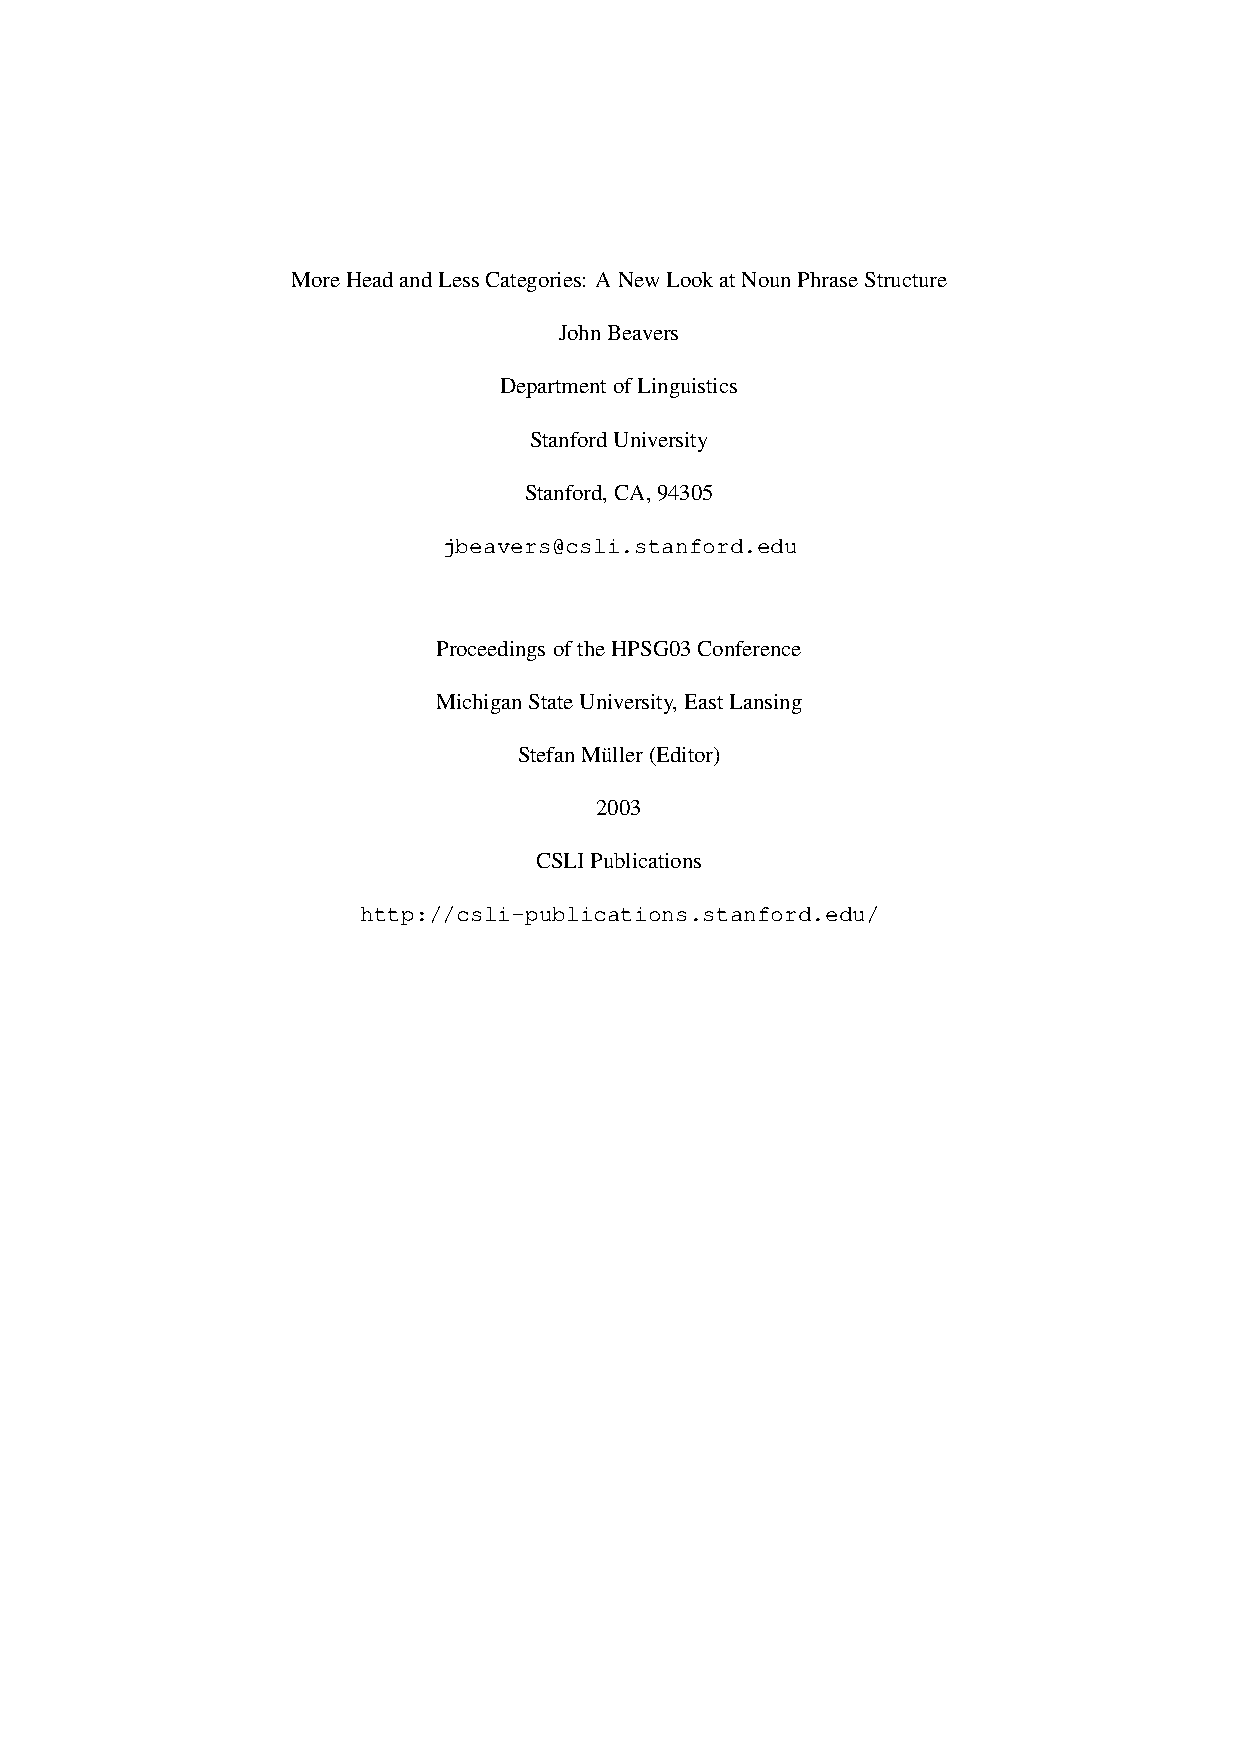
\includepdf[pages=-,pagecommand=\thispagestyle{plain}]{Includes/beavers.pdf}
        \setcounter{page}{68}
        \phantomsection
        \addcontentsline{toc}{section}{Chan Chung, Jong-Bok Kim: Capturing Word Order Asymmetries in English}
\thispagestyle{empty}

\begin{center}
  {\huge\bfseries Capturing Word Order Asymmetries in English\par}

  \bigskip

~\\
\begingroup
\setlength{\leftskip}{0pt plus 1fill}
\setlength{\rightskip}{0pt plus 1fill}
\setlength{\parindent}{0pt}
\setlength{\parfillskip}{0pt}
  \formatauthor{Chan Chung}{\begin{tabular}{@{}c@{}}Dongseo University\end{tabular}}
\formatauthor{Jong-Bok Kim}{\begin{tabular}{@{}c@{}}Kyung Hee University\end{tabular}}

\par\endgroup

  \vspace*{8ex}

  Proceedings of the 10th International Conference on\par Head-Driven Phrase Structure Grammar

  \bigskip

  Michigan State University

  \medskip

  Stefan Müller (Editor)

  \medskip

  2003

  \medskip

%  CSLI Publications

  \medskip

  pages 68--87

  \medskip

%  \url{http://csli-publications.stanford.edu/HPSG/2003}
\end{center}
\vfill

\noindent



\vfill
\noindent
% APA Style
Chung, Chan, \& Kim, Jong-Bok. 2003. Capturing Word Order Asymmetries in English. In Müller, Stefan (Ed.), \emph{{Proceedings of the 10th International Conference on Head-Driven Phrase Structure Grammar, Michigan State University}},
68--87. DOI: \href{http://doi.org/10.21248/hpsg.2003.7}{10.21248/hpsg.2003.7}. \hfill\href{http://creativecommons.org/licenses/by/4.0/}{\includegraphics[height=.75em]{Includes/ccby-eps-converted-to.pdf}}

\newpage
\includepdf[pages=-,pagecommand=\thispagestyle{plain}]{Includes/chung-kim.pdf}
        \setcounter{page}{88}
        \phantomsection
        \addcontentsline{toc}{section}{Kordula De Kuthy, W. Detmar Meurers: Dealing with Optional Complements in HPSG-Based Grammar Implementations}
\thispagestyle{empty}

\begin{center}
  {\huge\bfseries Dealing with Optional Complements in HPSG-Based Grammar Implementations\par}

  \bigskip

~\\
\begingroup
\setlength{\leftskip}{0pt plus 1fill}
\setlength{\rightskip}{0pt plus 1fill}
\setlength{\parindent}{0pt}
\setlength{\parfillskip}{0pt}
  \formatauthor{Kordula De Kuthy}{\begin{tabular}{@{}c@{}}Ohio State University\end{tabular}}
\formatauthor{W. Detmar Meurers}{\begin{tabular}{@{}c@{}}Ohio State University\end{tabular}}

\par\endgroup

  \vspace*{8ex}

  Proceedings of the 10th International Conference on\par Head-Driven Phrase Structure Grammar

  \bigskip

  Michigan State University

  \medskip

  Stefan Müller (Editor)

  \medskip

  2003

  \medskip

%  CSLI Publications

  \medskip

  pages 88--96

  \medskip

%  \url{http://csli-publications.stanford.edu/HPSG/2003}
\end{center}
\vfill

\noindent



\vfill
\noindent
% APA Style
De Kuthy, Kordula, \& Meurers, W. Detmar. 2003. Dealing with Optional Complements in HPSG-Based Grammar Implementations. In Müller, Stefan (Ed.), \emph{{Proceedings of the 10th International Conference on Head-Driven Phrase Structure Grammar, Michigan State University}},
88--96. DOI: \href{http://doi.org/10.21248/hpsg.2003.8}{10.21248/hpsg.2003.8}. \hfill\href{http://creativecommons.org/licenses/by/4.0/}{\includegraphics[height=.75em]{Includes/ccby-eps-converted-to.pdf}}

\newpage
\includepdf[pages=-,pagecommand=\thispagestyle{plain}]{Includes/dekuthy-meurers.pdf}
        \setcounter{page}{97}
        \phantomsection
        \addcontentsline{toc}{section}{Kordula De Kuthy, W. Detmar Meurers: The Secret Life of Focus Exponents, and What it Tells Us about Fronted Verbal Projections}
\thispagestyle{empty}

\begin{center}
  {\huge\bfseries The Secret Life of Focus Exponents, and What it Tells Us about Fronted Verbal Projections\par}

  \bigskip

~\\
\begingroup
\setlength{\leftskip}{0pt plus 1fill}
\setlength{\rightskip}{0pt plus 1fill}
\setlength{\parindent}{0pt}
\setlength{\parfillskip}{0pt}
  \formatauthor{Kordula De Kuthy}{\begin{tabular}{@{}c@{}}Ohio State University\end{tabular}}
\formatauthor{W. Detmar Meurers}{\begin{tabular}{@{}c@{}}Ohio State University\end{tabular}}

\par\endgroup

  \vspace*{8ex}

  Proceedings of the 10th International Conference on\par Head-Driven Phrase Structure Grammar

  \bigskip

  Michigan State University

  \medskip

  Stefan Müller (Editor)

  \medskip

  2003

  \medskip

%  CSLI Publications

  \medskip

  pages 97--110

  \medskip

%  \url{http://csli-publications.stanford.edu/HPSG/2003}
\end{center}
\vfill

\noindent



\vfill
\noindent
% APA Style
De Kuthy, Kordula, \& Meurers, W. Detmar. 2003. The Secret Life of Focus Exponents, and What it Tells Us about Fronted Verbal Projections. In Müller, Stefan (Ed.), \emph{{Proceedings of the 10th International Conference on Head-Driven Phrase Structure Grammar, Michigan State University}},
97--110. DOI: \href{http://doi.org/10.21248/hpsg.2003.9}{10.21248/hpsg.2003.9}. \hfill\href{http://creativecommons.org/licenses/by/4.0/}{\includegraphics[height=.75em]{Includes/ccby-eps-converted-to.pdf}}

\newpage
\includepdf[pages=-,pagecommand=\thispagestyle{plain}]{Includes/dekuthy-meurers-2.pdf}
        \setcounter{page}{111}
        \phantomsection
        \addcontentsline{toc}{section}{Dan Flickinger, Francis Bond: A Two-Rule Analysis of Measure Noun Phrases}
\thispagestyle{empty}

\begin{center}
  {\huge\bfseries A Two-Rule Analysis of Measure Noun Phrases\par}

  \bigskip

~\\
\begingroup
\setlength{\leftskip}{0pt plus 1fill}
\setlength{\rightskip}{0pt plus 1fill}
\setlength{\parindent}{0pt}
\setlength{\parfillskip}{0pt}
  \formatauthor{Dan Flickinger}{\begin{tabular}{@{}c@{}}Stanford University\end{tabular}}
\formatauthor{Francis Bond}{\begin{tabular}{@{}c@{}}NTT Communication Science Labs\end{tabular}}

\par\endgroup

  \vspace*{8ex}

  Proceedings of the 10th International Conference on\par Head-Driven Phrase Structure Grammar

  \bigskip

  Michigan State University

  \medskip

  Stefan Müller (Editor)

  \medskip

  2003

  \medskip

%  CSLI Publications

  \medskip

  pages 111--121

  \medskip

%  \url{http://csli-publications.stanford.edu/HPSG/2003}
\end{center}
\vfill

\noindent



\vfill
\noindent
% APA Style
Flickinger, Dan, \& Bond, Francis. 2003. A Two-Rule Analysis of Measure Noun Phrases. In Müller, Stefan (Ed.), \emph{{Proceedings of the 10th International Conference on Head-Driven Phrase Structure Grammar, Michigan State University}},
111--121. DOI: \href{http://doi.org/10.21248/hpsg.2003.10}{10.21248/hpsg.2003.10}. \hfill\href{http://creativecommons.org/licenses/by/4.0/}{\includegraphics[height=.75em]{Includes/ccby-eps-converted-to.pdf}}

\newpage
\includepdf[pages=-,pagecommand=\thispagestyle{plain}]{Includes/flickinger-bond.pdf}
        \setcounter{page}{122}
        \phantomsection
        \addcontentsline{toc}{section}{Jeanette Gundel: Information Structure and Referential Givenness/Newness: How Much Belongs in the Grammar?}
\thispagestyle{empty}

\begin{center}
  {\huge\bfseries Information Structure and Referential Givenness/Newness: How Much Belongs in the Grammar?\par}

  \bigskip

~\\
\begingroup
\setlength{\leftskip}{0pt plus 1fill}
\setlength{\rightskip}{0pt plus 1fill}
\setlength{\parindent}{0pt}
\setlength{\parfillskip}{0pt}
  \formatauthor{Jeanette Gundel}{\begin{tabular}{@{}c@{}}University of Minnesota\end{tabular}}

\par\endgroup

  \vspace*{8ex}

  Proceedings of the 10th International Conference on\par Head-Driven Phrase Structure Grammar

  \bigskip

  Michigan State University

  \medskip

  Stefan Müller (Editor)

  \medskip

  2003

  \medskip

%  CSLI Publications

  \medskip

  pages 122--142

  \medskip

%  \url{http://csli-publications.stanford.edu/HPSG/2003}
\end{center}
\vfill

\noindent



\vfill
\noindent
% APA Style
Gundel, Jeanette. 2003. Information Structure and Referential Givenness/Newness: How Much Belongs in the Grammar? In Müller, Stefan (Ed.), \emph{{Proceedings of the 10th International Conference on Head-Driven Phrase Structure Grammar, Michigan State University}},
122--142. DOI: \href{http://doi.org/10.21248/hpsg.2003.11}{10.21248/hpsg.2003.11}. \hfill\href{http://creativecommons.org/licenses/by/4.0/}{\includegraphics[height=.75em]{Includes/ccby-eps-converted-to.pdf}}

\newpage
\includepdf[pages=-,pagecommand=\thispagestyle{plain}]{Includes/gundel.pdf}
        \setcounter{page}{143}
        \phantomsection
        \addcontentsline{toc}{section}{Mohammad Haji-Abdolhosseini: Constraint-Based Approach to Information Structure and Prosody Correspondence}
\thispagestyle{empty}

\begin{center}
  {\huge\bfseries Constraint-Based Approach to Information Structure and Prosody Correspondence\par}

  \bigskip

~\\
\begingroup
\setlength{\leftskip}{0pt plus 1fill}
\setlength{\rightskip}{0pt plus 1fill}
\setlength{\parindent}{0pt}
\setlength{\parfillskip}{0pt}
  \formatauthor{Mohammad Haji-Abdolhosseini}{\begin{tabular}{@{}c@{}}University of Toronto\end{tabular}}

\par\endgroup

  \vspace*{8ex}

  Proceedings of the 10th International Conference on\par Head-Driven Phrase Structure Grammar

  \bigskip

  Michigan State University

  \medskip

  Stefan Müller (Editor)

  \medskip

  2003

  \medskip

%  CSLI Publications

  \medskip

  pages 143--162

  \medskip

%  \url{http://csli-publications.stanford.edu/HPSG/2003}
\end{center}
\vfill

\noindent



\vfill
\noindent
% APA Style
Haji-Abdolhosseini, Mohammad. 2003. Constraint-Based Approach to Information Structure and Prosody Correspondence. In Müller, Stefan (Ed.), \emph{{Proceedings of the 10th International Conference on Head-Driven Phrase Structure Grammar, Michigan State University}},
143--162. DOI: \href{http://doi.org/10.21248/hpsg.2003.12}{10.21248/hpsg.2003.12}. \hfill\href{http://creativecommons.org/licenses/by/4.0/}{\includegraphics[height=.75em]{Includes/ccby-eps-converted-to.pdf}}

\newpage
\includepdf[pages=-,pagecommand=\thispagestyle{plain}]{Includes/haji-abdolhosseini.pdf}
        \setcounter{page}{163}
        \phantomsection
        \addcontentsline{toc}{section}{Anke Holler: An HPSG Analysis of the Non-Integrated \emph{Wh}-Relative Clauses in German}
\thispagestyle{empty}

\begin{center}
  {\huge\bfseries An HPSG Analysis of the Non-Integrated \emph{Wh}-Relative Clauses in German\par}

  \bigskip

~\\
\begingroup
\setlength{\leftskip}{0pt plus 1fill}
\setlength{\rightskip}{0pt plus 1fill}
\setlength{\parindent}{0pt}
\setlength{\parfillskip}{0pt}
  \formatauthor{Anke Holler}{\begin{tabular}{@{}c@{}}University of Heidelberg \\ TEMIS Deutschland\end{tabular}}

\par\endgroup

  \vspace*{8ex}

  Proceedings of the 10th International Conference on\par Head-Driven Phrase Structure Grammar

  \bigskip

  Michigan State University

  \medskip

  Stefan Müller (Editor)

  \medskip

  2003

  \medskip

%  CSLI Publications

  \medskip

  pages 163--180

  \medskip

%  \url{http://csli-publications.stanford.edu/HPSG/2003}
\end{center}
\vfill

\noindent



\vfill
\noindent
% APA Style
Holler, Anke. 2003. An HPSG Analysis of the Non-Integrated \emph{Wh}-Relative Clauses in German. In Müller, Stefan (Ed.), \emph{{Proceedings of the 10th International Conference on Head-Driven Phrase Structure Grammar, Michigan State University}},
163--180. DOI: \href{http://doi.org/10.21248/hpsg.2003.13}{10.21248/hpsg.2003.13}. \hfill\href{http://creativecommons.org/licenses/by/4.0/}{\includegraphics[height=.75em]{Includes/ccby-eps-converted-to.pdf}}

\newpage
\includepdf[pages=-,pagecommand=\thispagestyle{plain}]{Includes/holler.pdf}
        \setcounter{page}{181}
        \phantomsection
        \addcontentsline{toc}{section}{Florian Jaeger: Topics First! In- and Outside of Bulgarian \emph{Wh}-Interrogatives}
\thispagestyle{empty}

\begin{center}
  {\huge\bfseries Topics First! In- and Outside of Bulgarian \emph{Wh}-Interrogatives\par}

  \bigskip

~\\
\begingroup
\setlength{\leftskip}{0pt plus 1fill}
\setlength{\rightskip}{0pt plus 1fill}
\setlength{\parindent}{0pt}
\setlength{\parfillskip}{0pt}
  \formatauthor{Florian Jaeger}{\begin{tabular}{@{}c@{}}Stanford University\end{tabular}}

\par\endgroup

  \vspace*{8ex}

  Proceedings of the 10th International Conference on\par Head-Driven Phrase Structure Grammar

  \bigskip

  Michigan State University

  \medskip

  Stefan Müller (Editor)

  \medskip

  2003

  \medskip

%  CSLI Publications

  \medskip

  pages 181--202

  \medskip

%  \url{http://csli-publications.stanford.edu/HPSG/2003}
\end{center}
\vfill

\noindent



\vfill
\noindent
% APA Style
Jaeger, Florian. 2003. Topics First! In- and Outside of Bulgarian \emph{Wh}-Interrogatives. In Müller, Stefan (Ed.), \emph{{Proceedings of the 10th International Conference on Head-Driven Phrase Structure Grammar, Michigan State University}},
181--202. DOI: \href{http://doi.org/10.21248/hpsg.2003.14}{10.21248/hpsg.2003.14}. \hfill\href{http://creativecommons.org/licenses/by/4.0/}{\includegraphics[height=.75em]{Includes/ccby-eps-converted-to.pdf}}

\newpage
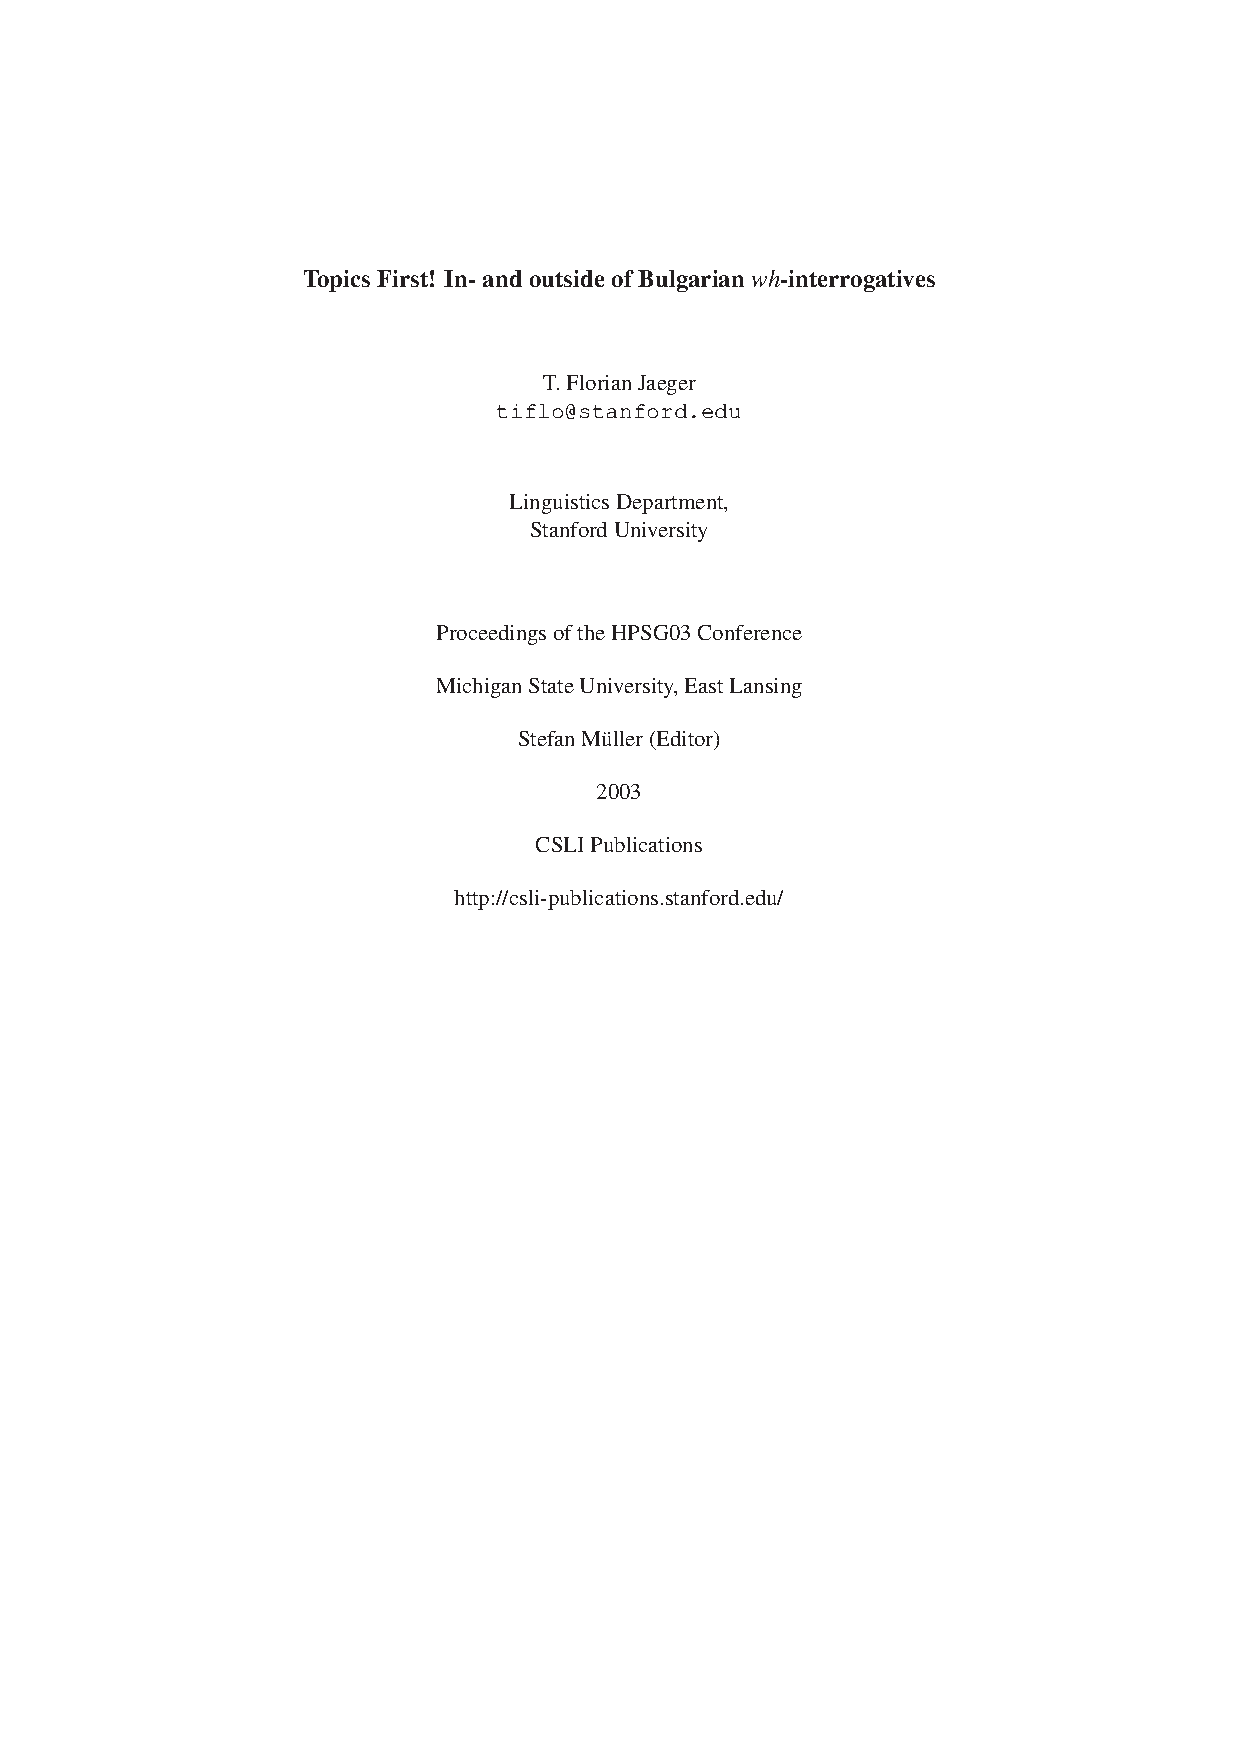
\includepdf[pages=-,pagecommand=\thispagestyle{plain}]{Includes/jaeger.pdf}
        \setcounter{page}{203}
        \phantomsection
        \addcontentsline{toc}{section}{Andreas Kathol: Cooperating Constructions in Lai ``Lexical Insertion''}
\thispagestyle{empty}

\begin{center}
  {\huge\bfseries Cooperating Constructions in Lai ``Lexical Insertion''\par}

  \bigskip

~\\
\begingroup
\setlength{\leftskip}{0pt plus 1fill}
\setlength{\rightskip}{0pt plus 1fill}
\setlength{\parindent}{0pt}
\setlength{\parfillskip}{0pt}
  \formatauthor{Andreas Kathol}{\begin{tabular}{@{}c@{}}University of California Berkeley\end{tabular}}

\par\endgroup

  \vspace*{8ex}

  Proceedings of the 10th International Conference on\par Head-Driven Phrase Structure Grammar

  \bigskip

  Michigan State University

  \medskip

  Stefan Müller (Editor)

  \medskip

  2003

  \medskip

%  CSLI Publications

  \medskip

  pages 203--221

  \medskip

%  \url{http://csli-publications.stanford.edu/HPSG/2003}
\end{center}
\vfill

\noindent



\vfill
\noindent
% APA Style
Kathol, Andreas. 2003. Cooperating Constructions in Lai ``Lexical Insertion''. In Müller, Stefan (Ed.), \emph{{Proceedings of the 10th International Conference on Head-Driven Phrase Structure Grammar, Michigan State University}},
203--221. DOI: \href{http://doi.org/10.21248/hpsg.2003.15}{10.21248/hpsg.2003.15}. \hfill\href{http://creativecommons.org/licenses/by/4.0/}{\includegraphics[height=.75em]{Includes/ccby-eps-converted-to.pdf}}

\newpage
\includepdf[pages=-,pagecommand=\thispagestyle{plain}]{Includes/kathol.pdf}
        \setcounter{page}{222}
        \phantomsection
        \addcontentsline{toc}{section}{Jean-Pierre Koenig, Anthony Davis: Semantically Transparent Linking in HPSG}
\thispagestyle{empty}

\begin{center}
  {\huge\bfseries Semantically Transparent Linking in HPSG\par}

  \bigskip

~\\
\begingroup
\setlength{\leftskip}{0pt plus 1fill}
\setlength{\rightskip}{0pt plus 1fill}
\setlength{\parindent}{0pt}
\setlength{\parfillskip}{0pt}
  \formatauthor{Jean-Pierre Koenig}{\begin{tabular}{@{}c@{}}University at Buffalo, SUNY\end{tabular}}
\formatauthor{Anthony Davis}{\begin{tabular}{@{}c@{}}University at Buffalo, SUNY\end{tabular}}

\par\endgroup

  \vspace*{8ex}

  Proceedings of the 10th International Conference on\par Head-Driven Phrase Structure Grammar

  \bigskip

  Michigan State University

  \medskip

  Stefan Müller (Editor)

  \medskip

  2003

  \medskip

%  CSLI Publications

  \medskip

  pages 222--235

  \medskip

%  \url{http://csli-publications.stanford.edu/HPSG/2003}
\end{center}
\vfill

\noindent



\vfill
\noindent
% APA Style
Koenig, Jean-Pierre, \& Davis, Anthony. 2003. Semantically Transparent Linking in HPSG. In Müller, Stefan (Ed.), \emph{{Proceedings of the 10th International Conference on Head-Driven Phrase Structure Grammar, Michigan State University}},
222--235. DOI: \href{http://doi.org/10.21248/hpsg.2003.16}{10.21248/hpsg.2003.16}. \hfill\href{http://creativecommons.org/licenses/by/4.0/}{\includegraphics[height=.75em]{Includes/ccby-eps-converted-to.pdf}}

\newpage
\includepdf[pages=-,pagecommand=\thispagestyle{plain}]{Includes/koenig-davis.pdf}
        \setcounter{page}{236}
        \phantomsection
        \addcontentsline{toc}{section}{Robert D. Levine, Ivan A. Sag: Some Empirical Issues in the Grammar of Extraction}
\thispagestyle{empty}

\begin{center}
  {\huge\bfseries Some Empirical Issues in the Grammar of Extraction\par}

  \bigskip

~\\
\begingroup
\setlength{\leftskip}{0pt plus 1fill}
\setlength{\rightskip}{0pt plus 1fill}
\setlength{\parindent}{0pt}
\setlength{\parfillskip}{0pt}
  \formatauthor{Robert D. Levine}{\begin{tabular}{@{}c@{}}Ohio State University\end{tabular}}
\formatauthor{Ivan A. Sag}{\begin{tabular}{@{}c@{}}Stanford University\end{tabular}}

\par\endgroup

  \vspace*{8ex}

  Proceedings of the 10th International Conference on\par Head-Driven Phrase Structure Grammar

  \bigskip

  Michigan State University

  \medskip

  Stefan Müller (Editor)

  \medskip

  2003

  \medskip

%  CSLI Publications

  \medskip

  pages 236--256

  \medskip

%  \url{http://csli-publications.stanford.edu/HPSG/2003}
\end{center}
\vfill

\noindent



\vfill
\noindent
% APA Style
Levine, Robert D., \& Sag, Ivan A. 2003. Some Empirical Issues in the Grammar of Extraction. In Müller, Stefan (Ed.), \emph{{Proceedings of the 10th International Conference on Head-Driven Phrase Structure Grammar, Michigan State University}},
236--256. DOI: \href{http://doi.org/10.21248/hpsg.2003.17}{10.21248/hpsg.2003.17}. \hfill\href{http://creativecommons.org/licenses/by/4.0/}{\includegraphics[height=.75em]{Includes/ccby-eps-converted-to.pdf}}

\newpage
\includepdf[pages=-,pagecommand=\thispagestyle{plain}]{Includes/levine-sag.pdf}
        \setcounter{page}{257}
        \phantomsection
        \addcontentsline{toc}{section}{Roger Levy, David Yoshikazu Oshima: Non-Transitive Information Flow in Japanese Noun-Classifier Matching}
\thispagestyle{empty}

\begin{center}
  {\huge\bfseries Non-Transitive Information Flow in Japanese Noun-Classifier Matching\par}

  \bigskip

~\\
\begingroup
\setlength{\leftskip}{0pt plus 1fill}
\setlength{\rightskip}{0pt plus 1fill}
\setlength{\parindent}{0pt}
\setlength{\parfillskip}{0pt}
  \formatauthor{Roger Levy}{\begin{tabular}{@{}c@{}}Stanford University\end{tabular}}
\formatauthor{David Yoshikazu Oshima}{\begin{tabular}{@{}c@{}}Stanford University\end{tabular}}

\par\endgroup

  \vspace*{8ex}

  Proceedings of the 10th International Conference on\par Head-Driven Phrase Structure Grammar

  \bigskip

  Michigan State University

  \medskip

  Stefan Müller (Editor)

  \medskip

  2003

  \medskip

%  CSLI Publications

  \medskip

  pages 257--277

  \medskip

%  \url{http://csli-publications.stanford.edu/HPSG/2003}
\end{center}
\vfill

\noindent



\vfill
\noindent
% APA Style
Levy, Roger, \& Oshima, David Yoshikazu. 2003. Non-Transitive Information Flow in Japanese Noun-Classifier Matching. In Müller, Stefan (Ed.), \emph{{Proceedings of the 10th International Conference on Head-Driven Phrase Structure Grammar, Michigan State University}},
257--277. DOI: \href{http://doi.org/10.21248/hpsg.2003.18}{10.21248/hpsg.2003.18}. \hfill\href{http://creativecommons.org/licenses/by/4.0/}{\includegraphics[height=.75em]{Includes/ccby-eps-converted-to.pdf}}

\newpage
\includepdf[pages=-,pagecommand=\thispagestyle{plain}]{Includes/levy-oshima.pdf}
        \setcounter{page}{278}
        \phantomsection
        \addcontentsline{toc}{section}{Stefan M{\"u}ller: Object-to-Subject-Raising and Lexical Rule: An Analysis of the German Passiv}
\thispagestyle{empty}

\begin{center}
  {\huge\bfseries Object-to-Subject-Raising and Lexical Rule: An Analysis of the German Passiv\par}

  \bigskip

~\\
\begingroup
\setlength{\leftskip}{0pt plus 1fill}
\setlength{\rightskip}{0pt plus 1fill}
\setlength{\parindent}{0pt}
\setlength{\parfillskip}{0pt}
  \formatauthor{Stefan Müller\,\orcidlink{0000-0003-4413-5313}}{\begin{tabular}{@{}c@{}}University of Bremen\end{tabular}}

\par\endgroup

  \vspace*{8ex}

  Proceedings of the 10th International Conference on\par Head-Driven Phrase Structure Grammar

  \bigskip

  Michigan State University

  \medskip

  Stefan Müller (Editor)

  \medskip

  2003

  \medskip

%  CSLI Publications

  \medskip

  pages 278--297

  \medskip

%  \url{http://csli-publications.stanford.edu/HPSG/2003}
\end{center}
\vfill

\noindent



\vfill
\noindent
% APA Style
Müller, Stefan. 2003. Object-to-Subject-Raising and Lexical Rule: An Analysis of the German Passiv. In Müller, Stefan (Ed.), \emph{{Proceedings of the 10th International Conference on Head-Driven Phrase Structure Grammar, Michigan State University}},
278--297. DOI: \href{http://doi.org/10.21248/hpsg.2003.21}{10.21248/hpsg.2003.21}. \hfill\href{http://creativecommons.org/licenses/by/4.0/}{\includegraphics[height=.75em]{Includes/ccby-eps-converted-to.pdf}}

\newpage
\includepdf[pages=-,pagecommand=\thispagestyle{plain}]{Includes/mueller.pdf}
        \setcounter{page}{298}
        \phantomsection
        \addcontentsline{toc}{section}{Luis Paris, Jean-Pierre Koenig: What Does It Mean to Be a Complement?}
\thispagestyle{empty}

\begin{center}
  {\huge\bfseries What Does It Mean to Be a Complement?\par}

  \bigskip

~\\
\begingroup
\setlength{\leftskip}{0pt plus 1fill}
\setlength{\rightskip}{0pt plus 1fill}
\setlength{\parindent}{0pt}
\setlength{\parfillskip}{0pt}
  \formatauthor{Luis Paris}{\begin{tabular}{@{}c@{}}University at Albany, SUNY\end{tabular}}
\formatauthor{Jean-Pierre Koenig}{\begin{tabular}{@{}c@{}}University at Buffalo, SUNY\end{tabular}}

\par\endgroup

  \vspace*{8ex}

  Proceedings of the 10th International Conference on\par Head-Driven Phrase Structure Grammar

  \bigskip

  Michigan State University

  \medskip

  Stefan Müller (Editor)

  \medskip

  2003

  \medskip

%  CSLI Publications

  \medskip

  pages 298--317

  \medskip

%  \url{http://csli-publications.stanford.edu/HPSG/2003}
\end{center}
\vfill

\noindent



\vfill
\noindent
% APA Style
Paris, Luis, \& Koenig, Jean-Pierre. 2003. What Does It Mean to Be a Complement? In Müller, Stefan (Ed.), \emph{{Proceedings of the 10th International Conference on Head-Driven Phrase Structure Grammar, Michigan State University}},
298--317. DOI: \href{http://doi.org/10.21248/hpsg.2003.22}{10.21248/hpsg.2003.22}. \hfill\href{http://creativecommons.org/licenses/by/4.0/}{\includegraphics[height=.75em]{Includes/ccby-eps-converted-to.pdf}}

\newpage
\includepdf[pages=-,pagecommand=\thispagestyle{plain}]{Includes/paris-koenig.pdf}
        \setcounter{page}{318}
        \phantomsection
        \addcontentsline{toc}{section}{Gerald Penn, Kenneth Hoetmer: In Search of Epistemic Primitives in the English Resource Grammar (or Why HPSG Can't Live without Higher-Order Datatypes)}
\thispagestyle{empty}

\begin{center}
  {\huge\bfseries In Search of Epistemic Primitives in the English Resource Grammar (or Why HPSG Can't Live without Higher-Order Datatypes)\par}

  \bigskip

~\\
\begingroup
\setlength{\leftskip}{0pt plus 1fill}
\setlength{\rightskip}{0pt plus 1fill}
\setlength{\parindent}{0pt}
\setlength{\parfillskip}{0pt}
  \formatauthor{Gerald Penn}{\begin{tabular}{@{}c@{}}University of Toronto\end{tabular}}
\formatauthor{Kenneth Hoetmer}{\begin{tabular}{@{}c@{}}University of Toronto\end{tabular}}

\par\endgroup

  \vspace*{8ex}

  Proceedings of the 10th International Conference on\par Head-Driven Phrase Structure Grammar

  \bigskip

  Michigan State University

  \medskip

  Stefan Müller (Editor)

  \medskip

  2003

  \medskip

%  CSLI Publications

  \medskip

  pages 318--337

  \medskip

%  \url{http://csli-publications.stanford.edu/HPSG/2003}
\end{center}
\vfill

\noindent



\vfill
\noindent
% APA Style
Penn, Gerald, \& Hoetmer, Kenneth. 2003. In Search of Epistemic Primitives in the English Resource Grammar (or Why HPSG Can't Live without Higher-Order Datatypes). In Müller, Stefan (Ed.), \emph{{Proceedings of the 10th International Conference on Head-Driven Phrase Structure Grammar, Michigan State University}},
318--337. DOI: \href{http://doi.org/10.21248/hpsg.2003.23}{10.21248/hpsg.2003.23}. \hfill\href{http://creativecommons.org/licenses/by/4.0/}{\includegraphics[height=.75em]{Includes/ccby-eps-converted-to.pdf}}

\newpage
\includepdf[pages=-,pagecommand=\thispagestyle{plain}]{Includes/penn-hoetmer.pdf}
        \setcounter{page}{338}
        \phantomsection
        \addcontentsline{toc}{section}{Matthew Purver, Jonathan Ginzburg: Clarifying Noun Phrase Semantics in HPSG}
\thispagestyle{empty}

\begin{center}
  {\huge\bfseries Clarifying Noun Phrase Semantics in HPSG\par}

  \bigskip

~\\
\begingroup
\setlength{\leftskip}{0pt plus 1fill}
\setlength{\rightskip}{0pt plus 1fill}
\setlength{\parindent}{0pt}
\setlength{\parfillskip}{0pt}
  \formatauthor{Matthew Purver}{\begin{tabular}{@{}c@{}}King's College London\end{tabular}}
\formatauthor{Jonathan Ginzburg}{\begin{tabular}{@{}c@{}}King's College London\end{tabular}}

\par\endgroup

  \vspace*{8ex}

  Proceedings of the 10th International Conference on\par Head-Driven Phrase Structure Grammar

  \bigskip

  Michigan State University

  \medskip

  Stefan Müller (Editor)

  \medskip

  2003

  \medskip

%  CSLI Publications

  \medskip

  pages 338--358

  \medskip

%  \url{http://csli-publications.stanford.edu/HPSG/2003}
\end{center}
\vfill

\noindent



\vfill
\noindent
% APA Style
Purver, Matthew, \& Ginzburg, Jonathan. 2003. Clarifying Noun Phrase Semantics in HPSG. In Müller, Stefan (Ed.), \emph{{Proceedings of the 10th International Conference on Head-Driven Phrase Structure Grammar, Michigan State University}},
338--358. DOI: \href{http://doi.org/10.21248/hpsg.2003.24}{10.21248/hpsg.2003.24}. \hfill\href{http://creativecommons.org/licenses/by/4.0/}{\includegraphics[height=.75em]{Includes/ccby-eps-converted-to.pdf}}

\newpage
\includepdf[pages=-,pagecommand=\thispagestyle{plain}]{Includes/purver-ginzburg.pdf}
        \setcounter{page}{359}
        \phantomsection
        \addcontentsline{toc}{section}{Jeffrey T. Runner, Raul Aranovich: Noun Incorporation and Rule Interaction in the Lexicon}
\thispagestyle{empty}

\begin{center}
  {\huge\bfseries Noun Incorporation and Rule Interaction in the Lexicon\par}

  \bigskip

~\\
\begingroup
\setlength{\leftskip}{0pt plus 1fill}
\setlength{\rightskip}{0pt plus 1fill}
\setlength{\parindent}{0pt}
\setlength{\parfillskip}{0pt}
  \formatauthor{Jeffrey T. Runner}{\begin{tabular}{@{}c@{}}University of Rochester\end{tabular}}
\formatauthor{Raul Aranovich}{\begin{tabular}{@{}c@{}}University of California Davis\end{tabular}}

\par\endgroup

  \vspace*{8ex}

  Proceedings of the 10th International Conference on\par Head-Driven Phrase Structure Grammar

  \bigskip

  Michigan State University

  \medskip

  Stefan Müller (Editor)

  \medskip

  2003

  \medskip

%  CSLI Publications

  \medskip

  pages 359--379

  \medskip

%  \url{http://csli-publications.stanford.edu/HPSG/2003}
\end{center}
\vfill

\noindent



\vfill
\noindent
% APA Style
Runner, Jeffrey T., \& Aranovich, Raul. 2003. Noun Incorporation and Rule Interaction in the Lexicon. In Müller, Stefan (Ed.), \emph{{Proceedings of the 10th International Conference on Head-Driven Phrase Structure Grammar, Michigan State University}},
359--379. DOI: \href{http://doi.org/10.21248/hpsg.2003.25}{10.21248/hpsg.2003.25}. \hfill\href{http://creativecommons.org/licenses/by/4.0/}{\includegraphics[height=.75em]{Includes/ccby-eps-converted-to.pdf}}

\newpage
\includepdf[pages=-,pagecommand=\thispagestyle{plain}]{Includes/runner-aranovich.pdf}
        \setcounter{page}{380}
        \phantomsection
        \addcontentsline{toc}{section}{David Schlangen, Alex Lascarides: A Compositional and Constraint-Based Approach to Non-Sentential Utterances}
\thispagestyle{empty}

\begin{center}
  {\huge\bfseries A Compositional and Constraint-Based Approach to Non-Sentential Utterances\par}

  \bigskip

~\\
\begingroup
\setlength{\leftskip}{0pt plus 1fill}
\setlength{\rightskip}{0pt plus 1fill}
\setlength{\parindent}{0pt}
\setlength{\parfillskip}{0pt}
  \formatauthor{David Schlangen}{\begin{tabular}{@{}c@{}}University of Edinburgh\end{tabular}}
\formatauthor{Alex Lascarides}{\begin{tabular}{@{}c@{}}University of Edinburgh\end{tabular}}

\par\endgroup

  \vspace*{8ex}

  Proceedings of the 10th International Conference on\par Head-Driven Phrase Structure Grammar

  \bigskip

  Michigan State University

  \medskip

  Stefan Müller (Editor)

  \medskip

  2003

  \medskip

%  CSLI Publications

  \medskip

  pages 380--390

  \medskip

%  \url{http://csli-publications.stanford.edu/HPSG/2003}
\end{center}
\vfill

\noindent



\vfill
\noindent
% APA Style
Schlangen, David, \& Lascarides, Alex. 2003. A Compositional and Constraint-Based Approach to Non-Sentential Utterances. In Müller, Stefan (Ed.), \emph{{Proceedings of the 10th International Conference on Head-Driven Phrase Structure Grammar, Michigan State University}},
380--390. DOI: \href{http://doi.org/10.21248/hpsg.2003.26}{10.21248/hpsg.2003.26}. \hfill\href{http://creativecommons.org/licenses/by/4.0/}{\includegraphics[height=.75em]{Includes/ccby-eps-converted-to.pdf}}

\newpage
\includepdf[pages=-,pagecommand=\thispagestyle{plain}]{Includes/schlangen-lascarides.pdf}
        \setcounter{page}{391}
        \phantomsection
        \addcontentsline{toc}{section}{Frank Van Eynde: On the Notion `Determiner'}
\thispagestyle{empty}

\begin{center}
  {\huge\bfseries On the Notion `Determiner'\par}

  \bigskip

~\\
\begingroup
\setlength{\leftskip}{0pt plus 1fill}
\setlength{\rightskip}{0pt plus 1fill}
\setlength{\parindent}{0pt}
\setlength{\parfillskip}{0pt}
  \formatauthor{Frank Van Eynde}{\begin{tabular}{@{}c@{}}University of Leuven\end{tabular}}

\par\endgroup

  \vspace*{8ex}

  Proceedings of the 10th International Conference on\par Head-Driven Phrase Structure Grammar

  \bigskip

  Michigan State University

  \medskip

  Stefan Müller (Editor)

  \medskip

  2003

  \medskip

%  CSLI Publications

  \medskip

  pages 391--396

  \medskip

%  \url{http://csli-publications.stanford.edu/HPSG/2003}
\end{center}
\vfill

\noindent



\vfill
\noindent
% APA Style
Van Eynde, Frank. 2003. On the Notion `Determiner'. In Müller, Stefan (Ed.), \emph{{Proceedings of the 10th International Conference on Head-Driven Phrase Structure Grammar, Michigan State University}},
391--396. DOI: \href{http://doi.org/10.21248/hpsg.2003.29}{10.21248/hpsg.2003.29}. \hfill\href{http://creativecommons.org/licenses/by/4.0/}{\includegraphics[height=.75em]{Includes/ccby-eps-converted-to.pdf}}

\newpage
\includepdf[pages=-,pagecommand=\thispagestyle{plain}]{Includes/vaneynde.pdf}
        \setcounter{page}{397}
        \phantomsection
        \addcontentsline{toc}{section}{Eun-Jung Yoo: Specificational Pseudoclefts in English}
\thispagestyle{empty}

\begin{center}
  {\huge\bfseries Specificational Pseudoclefts in English\par}

  \bigskip

~\\
\begingroup
\setlength{\leftskip}{0pt plus 1fill}
\setlength{\rightskip}{0pt plus 1fill}
\setlength{\parindent}{0pt}
\setlength{\parfillskip}{0pt}
  \formatauthor{Eun-Jung Yoo}{\begin{tabular}{@{}c@{}}Seoul National University\end{tabular}}

\par\endgroup

  \vspace*{8ex}

  Proceedings of the 10th International Conference on\par Head-Driven Phrase Structure Grammar

  \bigskip

  Michigan State University

  \medskip

  Stefan Müller (Editor)

  \medskip

  2003

  \medskip

%  CSLI Publications

  \medskip

  pages 397--416

  \medskip

%  \url{http://csli-publications.stanford.edu/HPSG/2003}
\end{center}
\vfill

\noindent



\vfill
\noindent
% APA Style
Yoo, Eun-Jung. 2003. Specificational Pseudoclefts in English. In Müller, Stefan (Ed.), \emph{{Proceedings of the 10th International Conference on Head-Driven Phrase Structure Grammar, Michigan State University}},
397--416. DOI: \href{http://doi.org/10.21248/hpsg.2003.30}{10.21248/hpsg.2003.30}. \hfill\href{http://creativecommons.org/licenses/by/4.0/}{\includegraphics[height=.75em]{Includes/ccby-eps-converted-to.pdf}}

\newpage
\includepdf[pages=-,pagecommand=\thispagestyle{plain}]{Includes/yoo.pdf}
\end{document}
